\section{What is ML?}

Machine learning is the field of study responsible for developing and understanding algorithms that allow computer systems to perform certain tasks independently. The type of tasks considered are these for which any rule-based approach is unfeasible, either because a precise set of rules is unclear, for example in pattern recognition, or because computing according to the rules is too complex, for example in playing Go. 

Given a data set, the goal of a machine learning method can be of two types, one is to use the data to find a function, which will then match new input data to a value; another is to find a subdivision of the data set based on similarities. The methods used for the first type of goal are named \textit{supervised learning} methods and the given data set, called \textit{training set}, must be structured in pairs input-output. For the second type of goal, one uses \textit{unsupervised learning} methods.  

In a supervised learning method, the output value is either quantitative or qualitative. For the problem of predicting the price of house given its area and location, the output is a quantitative value; these are called \textit{regression} problems. On the other hand, if the task is to address an emotion to a given face expression, the output is a qualitative value encoding a certain emotion; these are called \textit{classification} problems.

Supervised learning methods are structured in two parts. Firstly it consists of a predetermined set of functions, called \textit{hypothesis space}, from which a final function will be chosen. Secondly the method needs a predetermined way of searching through the hypothesis space, therefore it requires a predetermined \textit{loss function} and \textit{optimization algorithm}. The choice of hypothesis space, loss function and optimization algorithm depends on the task and different methods need to be implemented and evaluated. For the task of recognizing facial emotion, it is known that between the methods so far developed, the best results are achieved by convolutional neural networks. Still, this project tests different methods one more time, for the sake of experience.

\begin{figure}[hbtp]
	\centering
	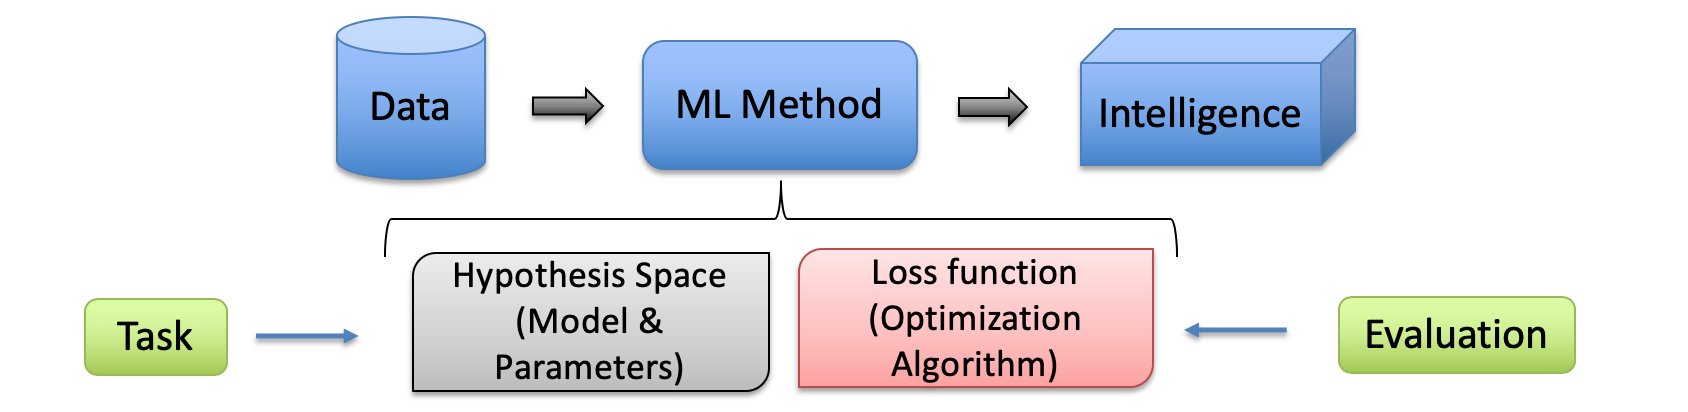
\includegraphics[width=1\textwidth]{./Images/MLPipe}
	\caption{The flow of developing an engine based on machine learning.}
	% \vspace{-20pt}
	\label{fig:Datensatz - unbearbeitet}
\end{figure}

%%%%%%%%%%%%%%%%%%%%%%%%%%%%%%%%%%%%%%%%%%%%%%%%%%%%%%%%%

\subsection{A first approach to Machine Learning: Linear Regression}

Machine Learning is not a new paradigm for developing algorithms, however the field's growing pace increased drastically in the 1990s. This was when the computational power and volume of available data finally allowed practical research. Due to this fast and recent development, multiple methods emerged without an established theory and organization as a base. For that reason, giving a brief overview on the most common algorithms can be a debatable and overwhelming task. 

\begin{figure}[hbtp]
	\centering
	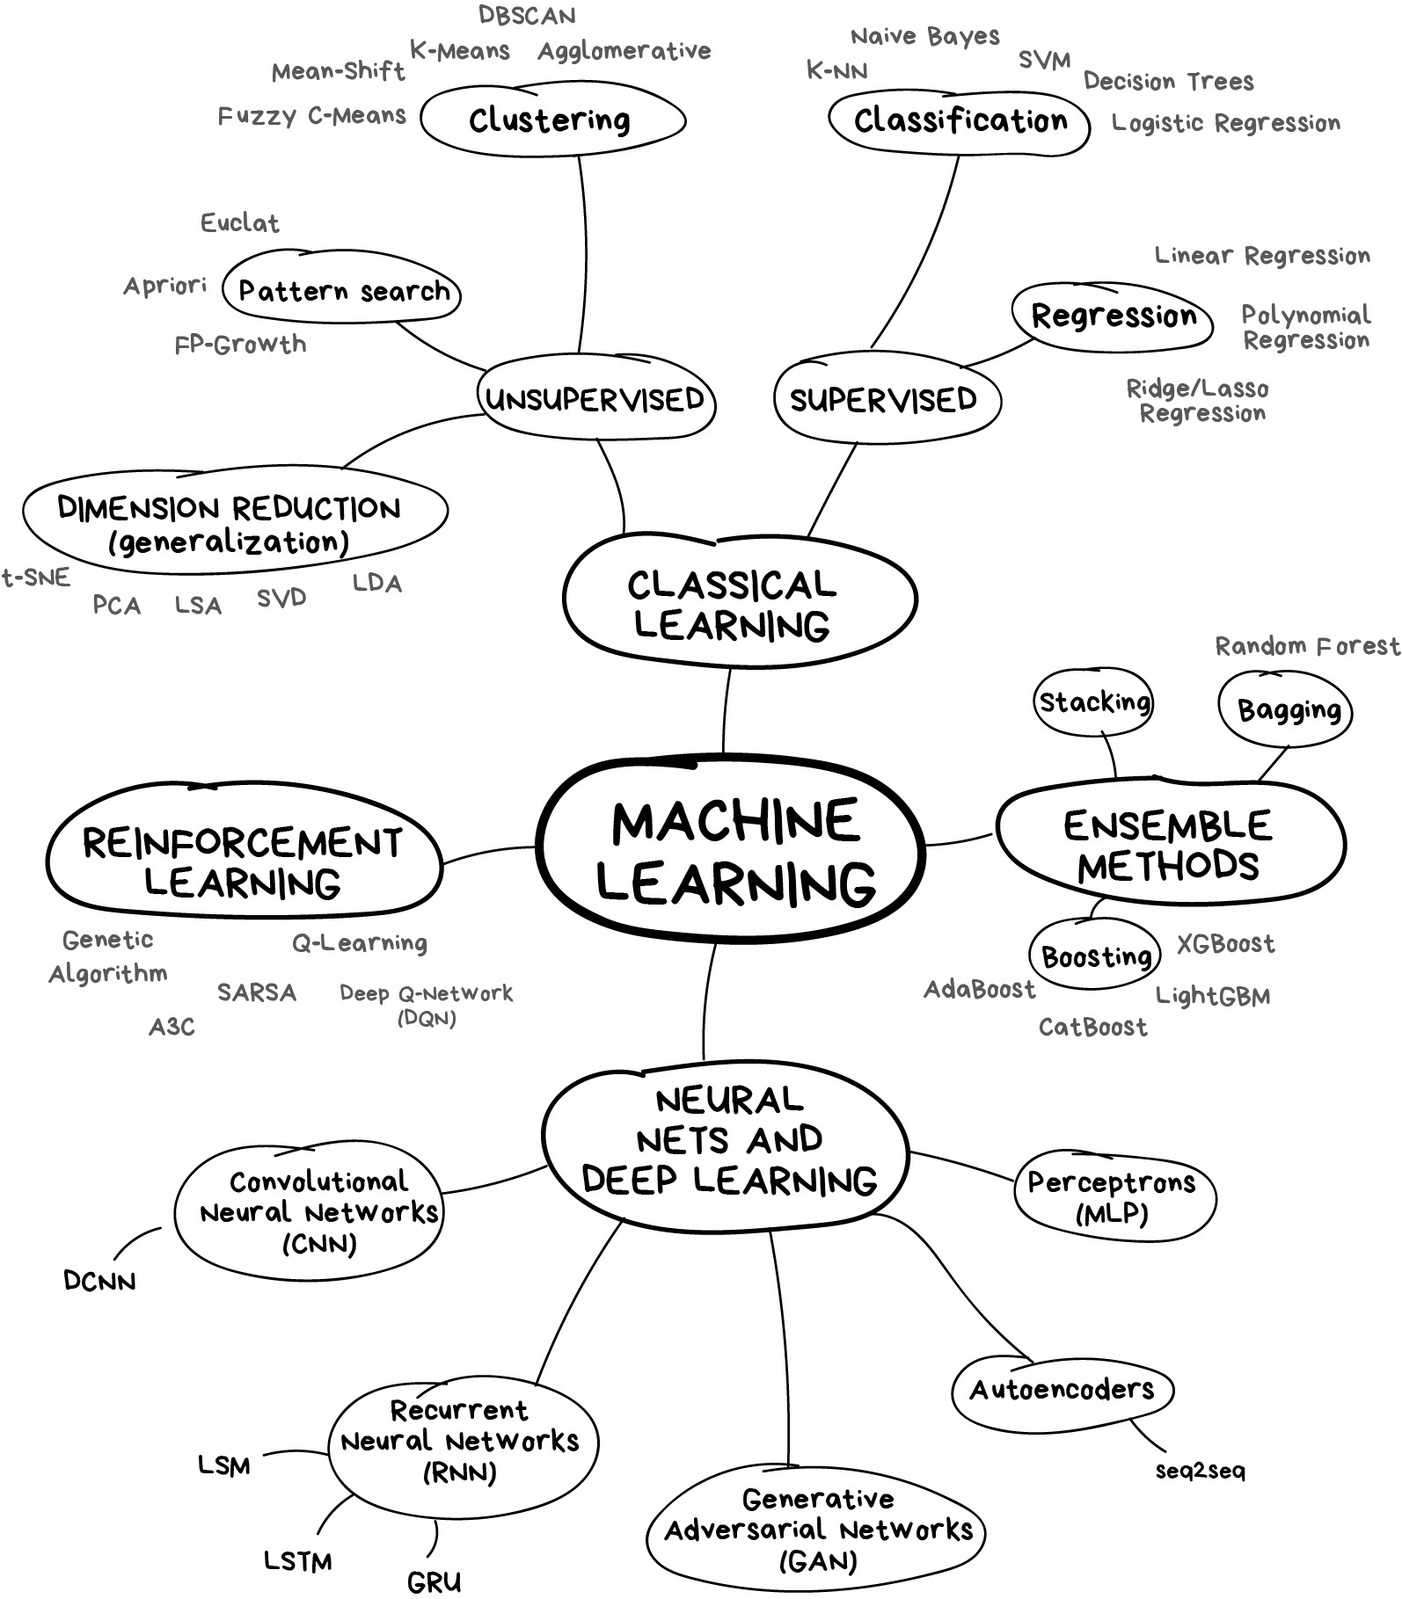
\includegraphics[width=1\textwidth]{ML}
	\caption{ML-Overview}
	% \vspace{-20pt}
	\label{fig:Datensatz - unbearbeitet}
\end{figure}

Nevertheless, giving the idea of some machine learning methods is still an interesting way to stablish a more concrete understanding of the field. In this section we give a brief overview on Linear Regression as an introductory example. 

In the following chapters we discuss $K$-Nearest Neighbours, Support Vector Machines,  Decision Trees, AdaBoost and Neural Networks.

\subsubsection{Linear Regression}
In a linear regression algorithm, the hypothesis space~$\mathcal{H}$ are functions~$h: \mathcal{X} \rightarrow \mathcal{Y}$ of shape
\[
h(x_1, \dots, x_d) = \beta_0 + \beta_1x_1 + \dots + \beta_dx_d,
\]
where the values~$\beta_i$ are parameters to be chosen. 

Given a data set~$\{(x^1, y^1), \dots, (x^n, y^n)\} \subset \mathcal{X} \times \mathcal{Y}$ of input-output pairs, a common choice of loss-function in regression problems is the square error given by
\[
L(h(x), y) = (h(x) - y)^2.
\]
This is a way of measuring the mismatch between the predicted output~$h(x^i)$ and the correct output~$y^i$.

For the choice of a final function, it's best to consider the whole set of training data, therefore define the empirical risk
\[
\hat{R}(h) = \frac{1}{n} \sum_{i = 1}^{n} L(h(x^i), y^i),
\]  
which averages the total mismatch. 

Finally, an optimization algorithm is used to solve the problem
\[
\underset{h \in \mathcal{H}}{\text{minimize}} \hat{R}(h).
\]
In this step, it is important that the empirical risk is a differentiable (or at least continuous) function.

\textbf{Notes}

This same approach can be used for a hypothesis space~$\mathcal{H}$ consisting of another type of (non-linear) functions, for example polynomials. If the functions in~$\mathcal{H}$ are also determined by few parameters, a minimizer might be found using methods from numerical optimization.

Also, this approach can be used with different loss-functions. A desirable loss-function could be the indicator
\[
L(h(x), y) = \mathds{1}_{\{h(x) = y\}} = \left\{ \begin{array}{lr}
1, & \text{if } h(x) = y\\
0, & \text{if } h(x)\neq y
\end{array} \right. .
\]
Nevertheless, this function is not continuous. Therefore one might look for ways os approximating it. 

In the case of a binary classifier, i.e.,~$\mathcal{Y} = \{0, 1\}$, a continuous approximation is the log-loss or cross-entropy function
\[
L(h(x), y) = \left\{ 
\begin{array}{lr}
-\log (h(x)), & \text{if } y = 1\\
-\log (1 - h(x)), & \text{if } y = 0
\end{array} \right. ,
\]
this gives large values when~$h(x)$ and~$y$ mismatch.




%%%%%%%%%%%%%%%%%%%%%%%%%%%%%%%%%%%%%%%%%%%%%%%%%%%%%%%%%

\subsection{The training Data}
TBA





\newpage